\documentclass[a4paper,14pt]{extarticle} 
\usepackage[a4paper,top=1.5cm, bottom=1.5cm, left=2cm, right=1cm]{geometry}
%\usepackage[T2A]{fontenc}
%\usepackage[english, russian]{babel}
\usepackage{graphicx}
\DeclareGraphicsExtensions{.pdf,.png,.jpg}

\usepackage{fontspec}
\setmainfont{Times New Roman}
\setsansfont{FreeSans}
\setmonofont{FreeMono}
\renewcommand{\baselinestretch}{1.5}
\usepackage{polyglossia}
\setdefaultlanguage{russian}
\setotherlanguages{english,russian}
\usepackage{setspace}
\usepackage[many]{tcolorbox}
\usepackage{listings}
\usepackage{xcolor}

\definecolor{codegreen}{rgb}{0,0.6,0}
\definecolor{codegray}{rgb}{0.5,0.5,0.5}
\definecolor{codepurple}{rgb}{0.58,0,0.82}
\definecolor{backcolour}{rgb}{0.95,0.95,0.92}

\lstdefinestyle{mystyle}{
    backgroundcolor=\color{backcolour},   
    keywordstyle=\color{magenta},
    numberstyle=\tiny\color{codegray},
    stringstyle=\color{codepurple},
    basicstyle=\ttfamily\footnotesize,
    breakatwhitespace=false,         
    breaklines=true,                 
    captionpos=b,                    
    keepspaces=true,                 
    numbers=left,                    
    numbersep=5pt,                  
    showspaces=false,                
    showstringspaces=false,
    showtabs=false,                  
    tabsize=2
}

\lstset{style=mystyle}
\setlength{\parindent}{5ex}


\begin{document}
    \begin{center}
        \thispagestyle{empty}
        \begin{singlespace}
        ФЕДЕРАЛЬНОЕ АГЕНТСТВО СВЯЗИ

        ФЕДЕРАЛЬНОЕ ГОСУДАРСТВЕННОЕ БЮДЖЕТНОЕ ОБРАЗОВАТЕЛЬНОЕ

        УЧРЕЖДЕНИЕ ВЫСШЕГО ОБРАЗОВАНИЯ

        «САНКТ-ПЕТЕРБУРГСКИЙ ГОСУДАРСТВЕННЫЙ УНИВЕРСИТЕТ ТЕЛЕКОММУНИКАЦИЙ ИМ. ПРОФ. М.А. БОНЧ-БРУЕВИЧА»

        (СПбГУТ)
        \end{singlespace}
        \vspace{-1ex}
        \rule{\textwidth}{0.4pt}
        \vspace{-5ex}

        Факультет \underline{Инфокоммуникационных сетей и систем}

        Кафедра \underline{Защищенных систем связи}
        \vspace{10ex}

        \textbf{Лаборатоoрная работа №2}\\
        МОНИТОРИНГ СЕТЕВОЙ И КОМПЬЮТЕРНОЙ АКТИВНОСТИ ПОЛЬЗОВАТЕЛЕЙ. Ч.1
        


    \end{center}
    \vspace{4ex}
    \begin{flushright}
    \parbox{10 cm}{
    \begin{flushleft}
        Выполнили студенты группы ИКТЗ-83:

        \underline{Громов А.А., Миколаени М.С., Мазеин Д.С.} \hfill \rule[-0.85ex]{0.1\textwidth}{0.6pt}

        \footnotesize \textit{ (Ф.И.О., № группы) \hfill (подпись)} \normalsize

        Проверил:

        \underline{Казанцев А.А.} \hfill \rule[-0.85ex]{0.1\textwidth}{0.6pt}

        (\footnotesize \textit{уч. степень, уч. звание, Ф.И.О.) \hfill (подпись)} \normalsize

    \end{flushleft}
    }
    \end{flushright}
    \begin{center}
        \vfill
        Санкт-Петербург

        2021

    \end{center}
    \newpage

    \textbf{Цель лабораторной работы:}

    Цель практического занятия: Научиться работе с Клиентской консолью
    Falcongaze SecureTower для проведения расследований и предупреждения инцидентов
    информационной безопасности организации, освоить различные виды поиска информации
    в объеме перехваченных данных. Научиться интерпретировать фотографию рабочего дня
    пользователя.

    \textbf{Пункт 2.2 - Изучение возможностей поиска}
    \begin{center}
        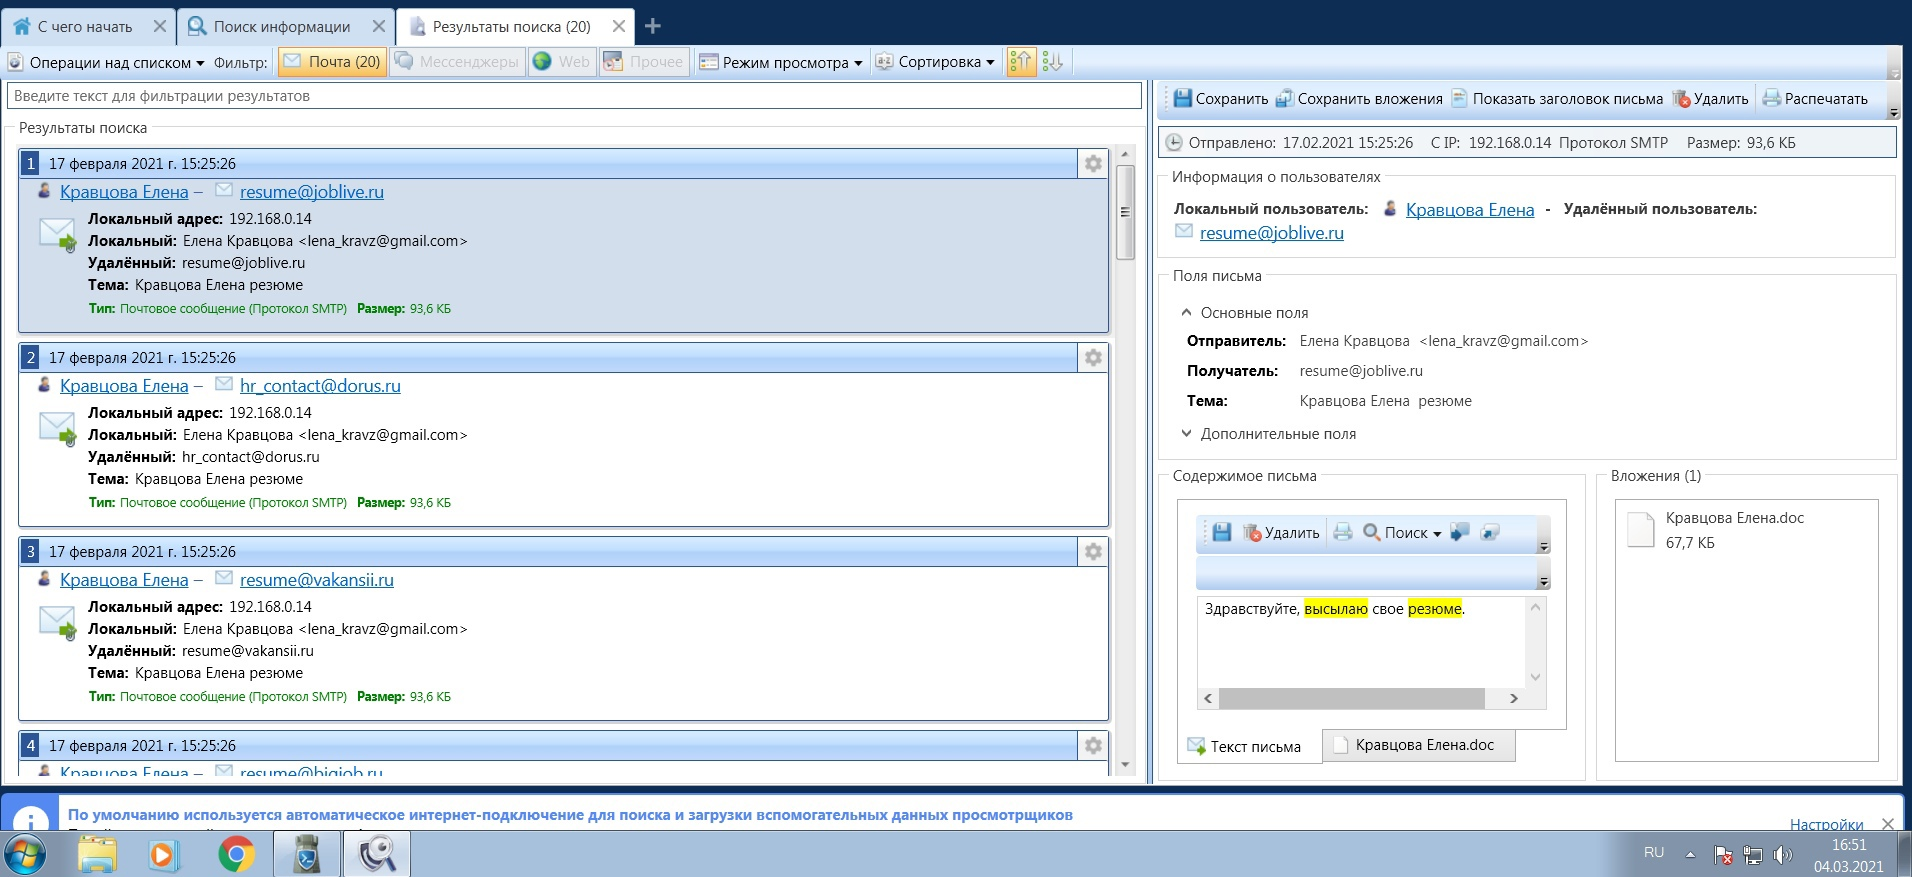
\includegraphics[scale=0.25]{pics/2.2.jpg}

        Результаты поиска
    \end{center}

    \textbf{Пункт 2.3 - Изучение возможностей поиска}
    \begin{center}
        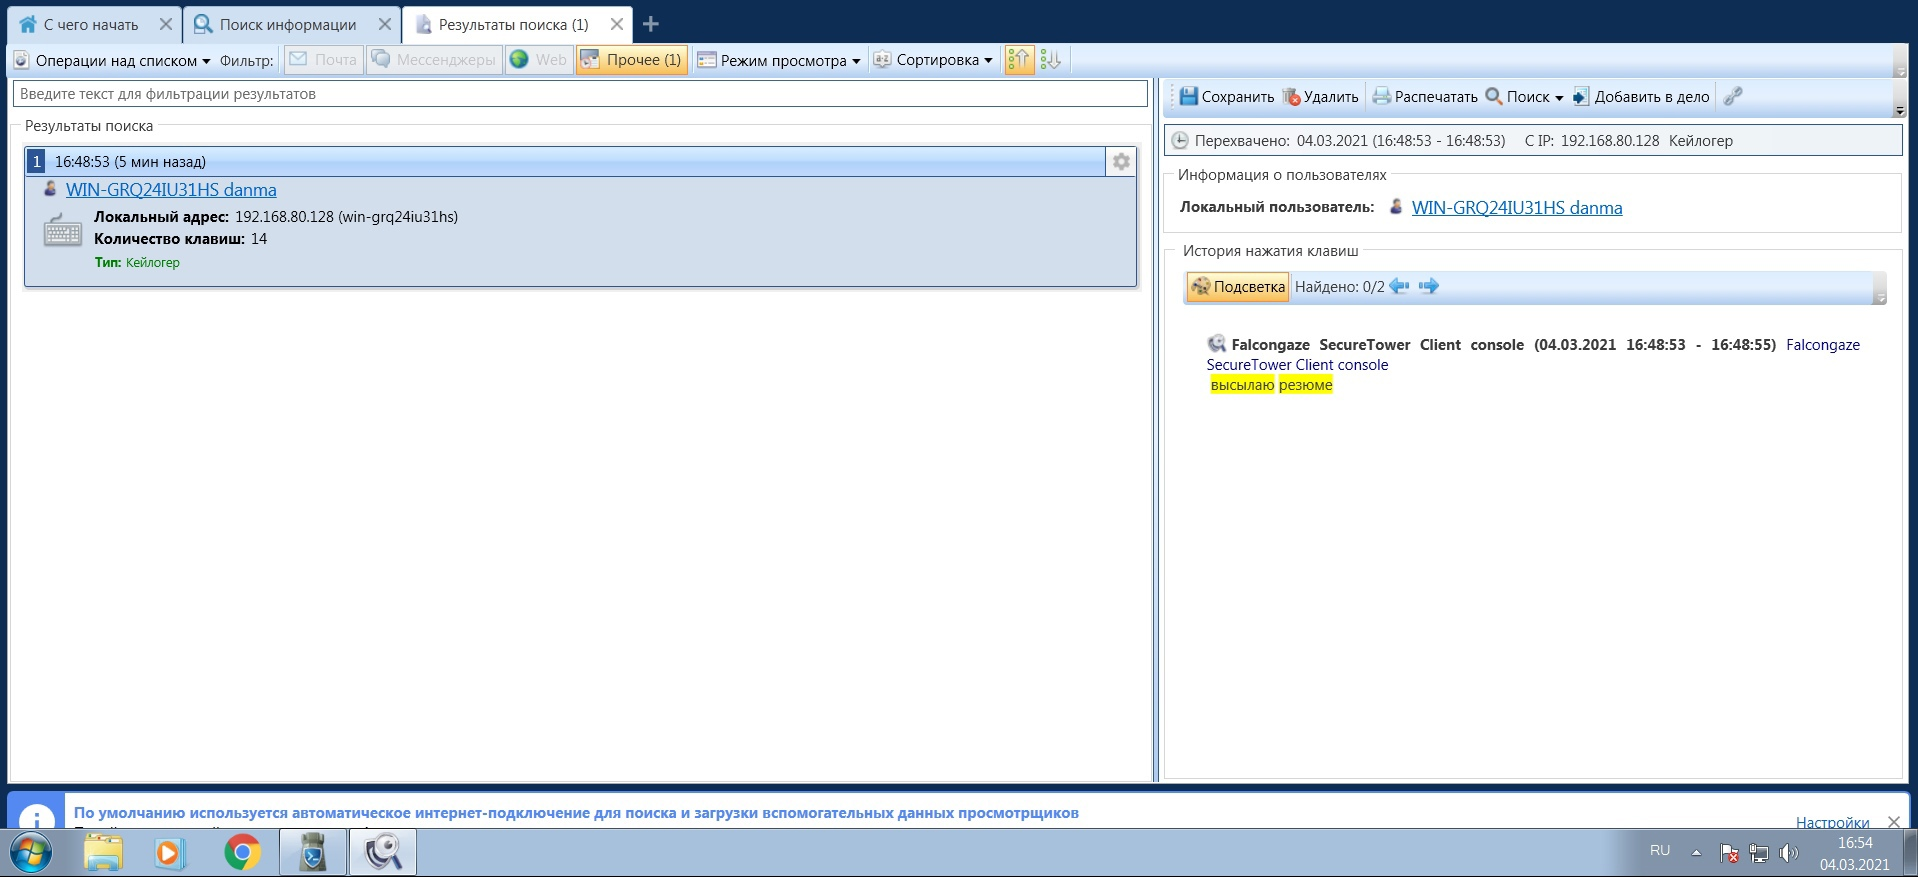
\includegraphics[scale=0.25]{pics/2.3.jpg}
        
        Найдено 1 совпадение.
    \end{center}

    \newpage
    \textbf{Пункт 2.4 - Изучение возможностей поиска}
    \begin{center}
        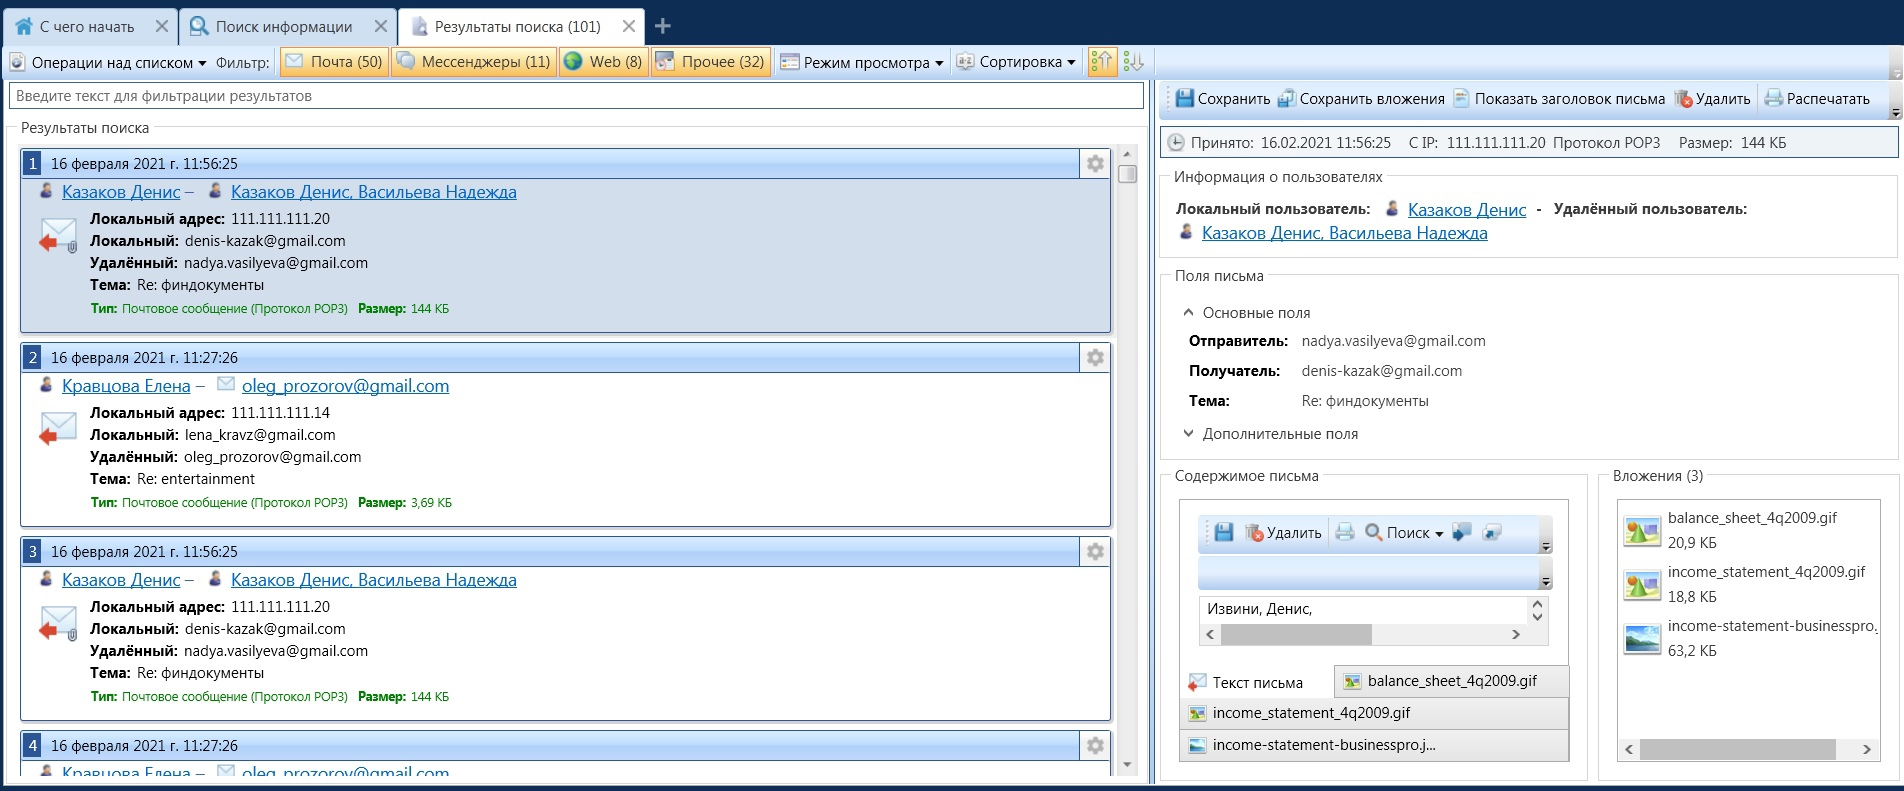
\includegraphics[scale=0.25]{pics/2.4.jpg}

        Найдено большое количество совпадение.
    \end{center}

    \textbf{Пункт 2.5 - Изучение возможностей поиска}
    \begin{center}
        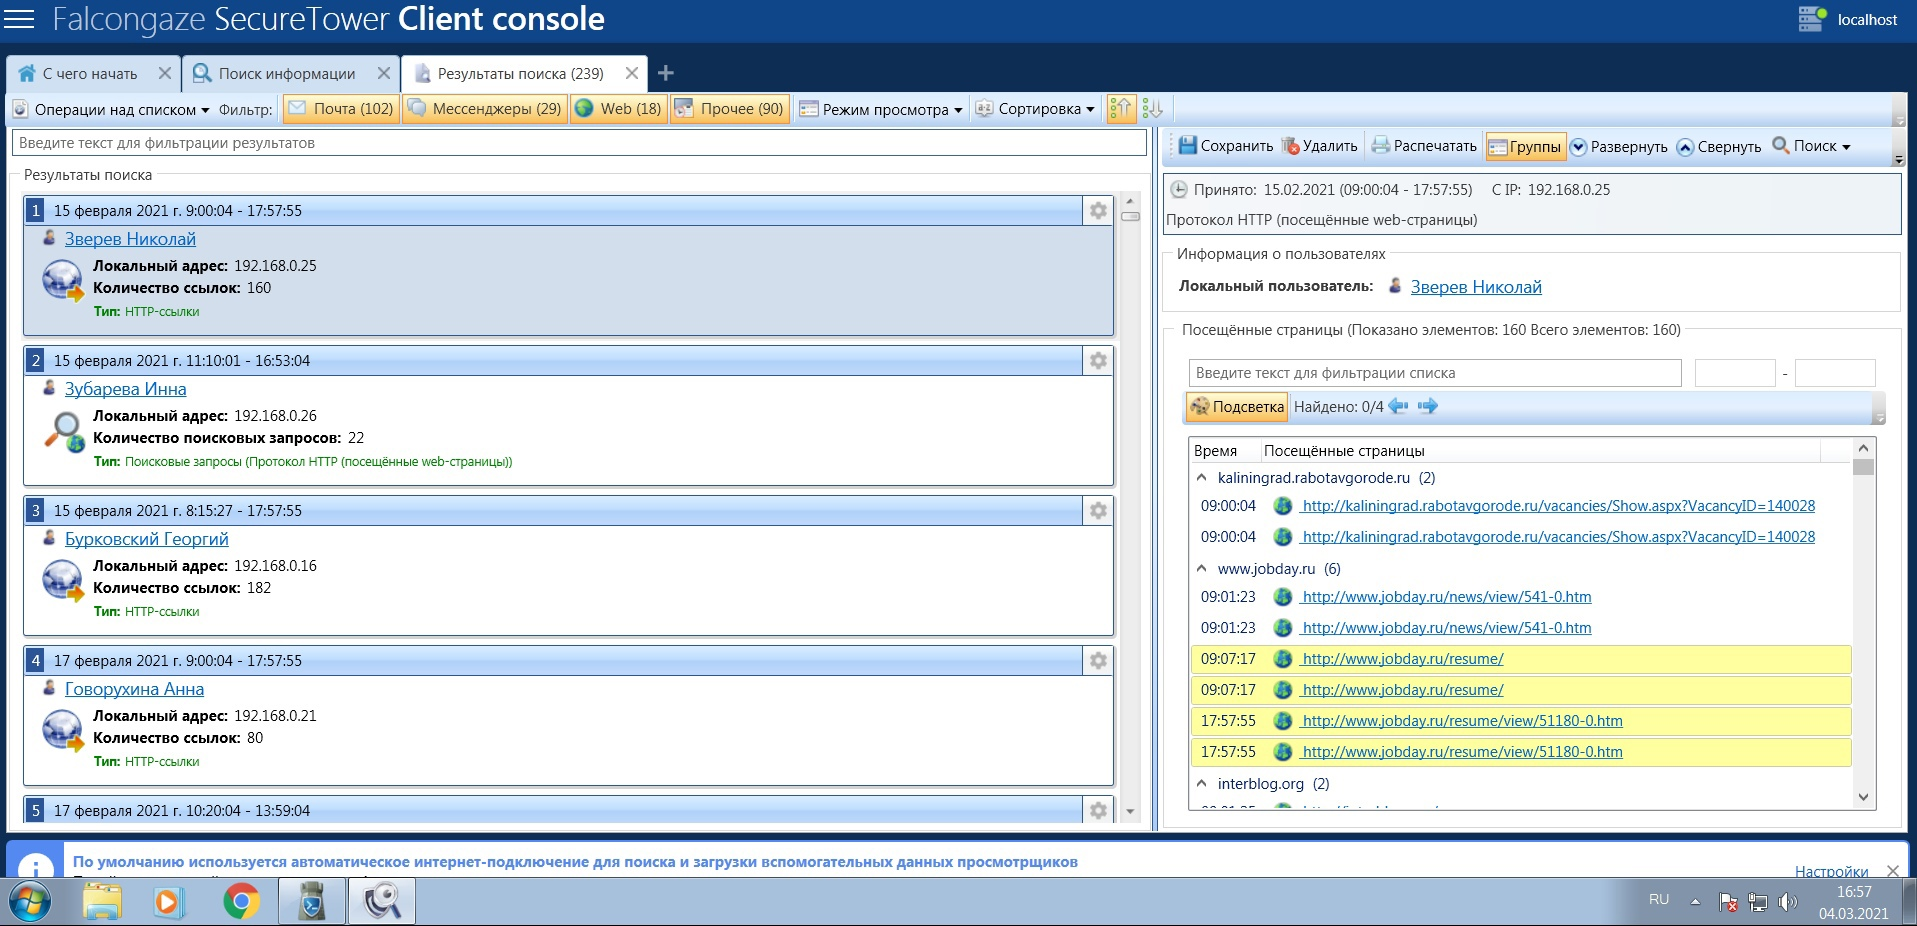
\includegraphics[scale=0.25]{pics/2.5.jpg}

        Найдено большое количество совпадение.
    \end{center}

    \newpage
    \textbf{Пункт 2.10 - Сохранение результатов в Excel}
    \begin{center}
        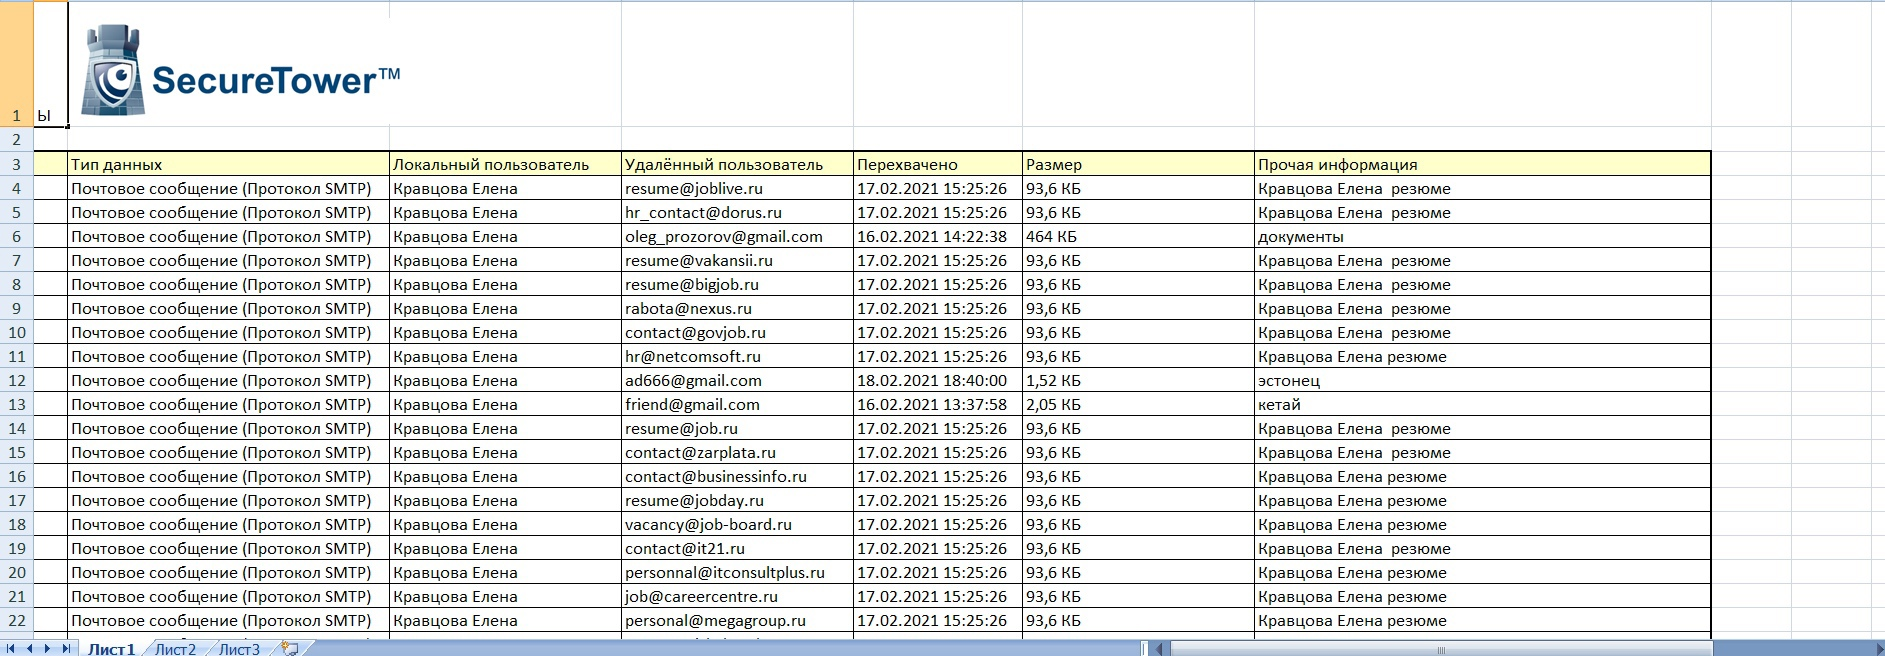
\includegraphics[scale=0.25]{pics/2.10.jpg}

        Таблица Excel
    \end{center}

    \textbf{Пункт 3.3 - Задайте поисковый запрос на обнаружение инцидентов передачи
    зашифрованных данных}
    \begin{center}
        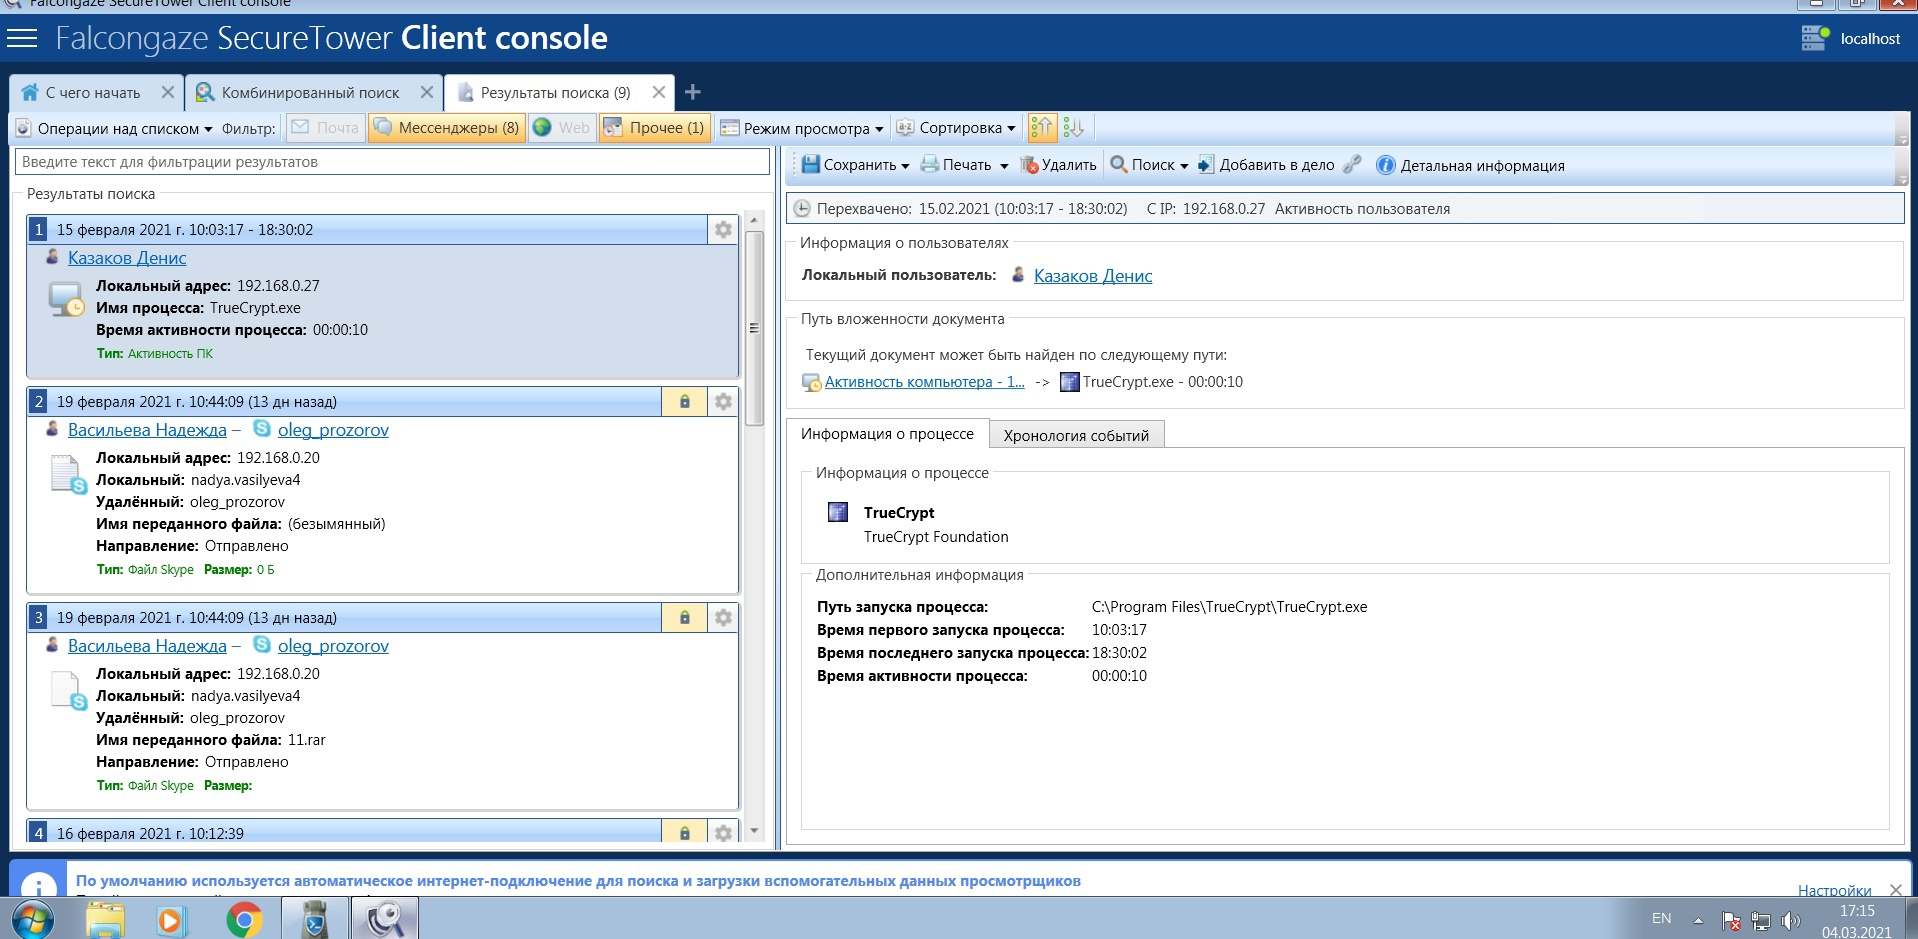
\includegraphics[scale=0.25]{pics/3.3.jpg}

        Обнаружена передача данных. 
    \end{center}

    \newpage
    \textbf{Пункт 3.6 - Связь удаленного пользователя Skype с локальным пользователем}
    \begin{center}
        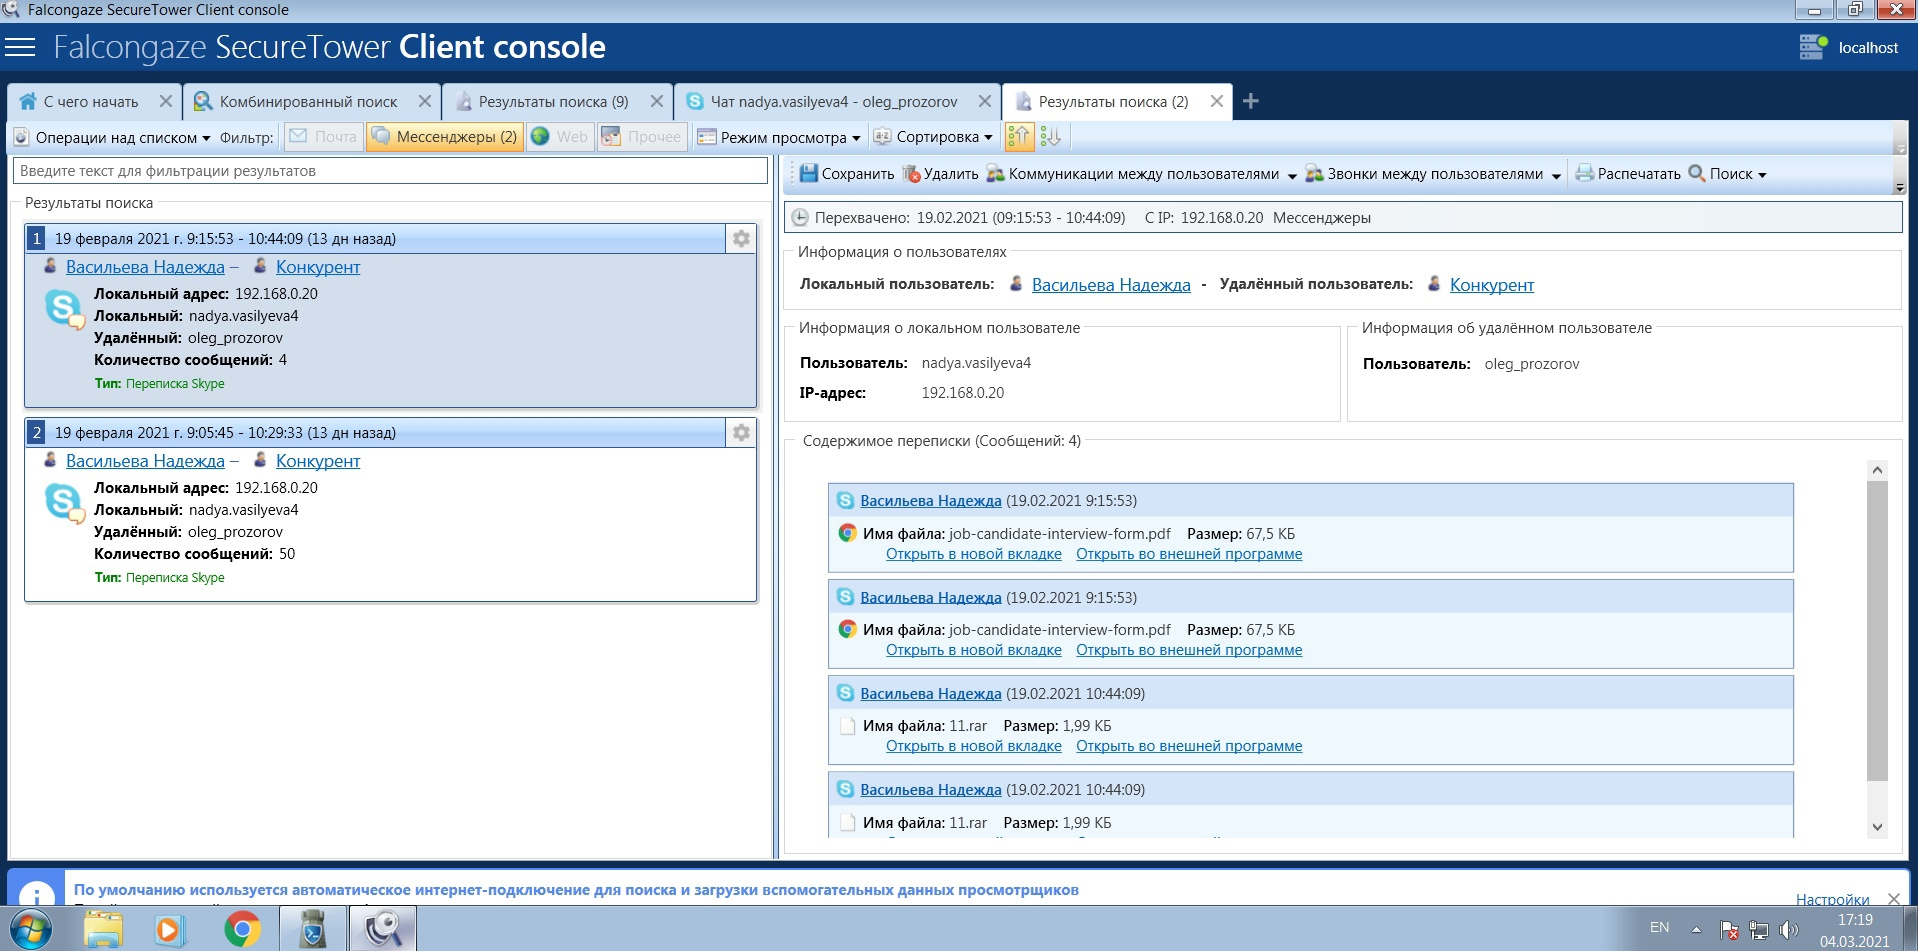
\includegraphics[scale=0.25]{pics/3.6.jpg}

        В окне Результаты поиска по коммуникациям имя контакта
        oleg\_prozorov заменено на Конкурент.
    \end{center}

    \textbf{Пункт 4.7 - Активация видео-аудио мониторинга.} 
    \begin{center}
        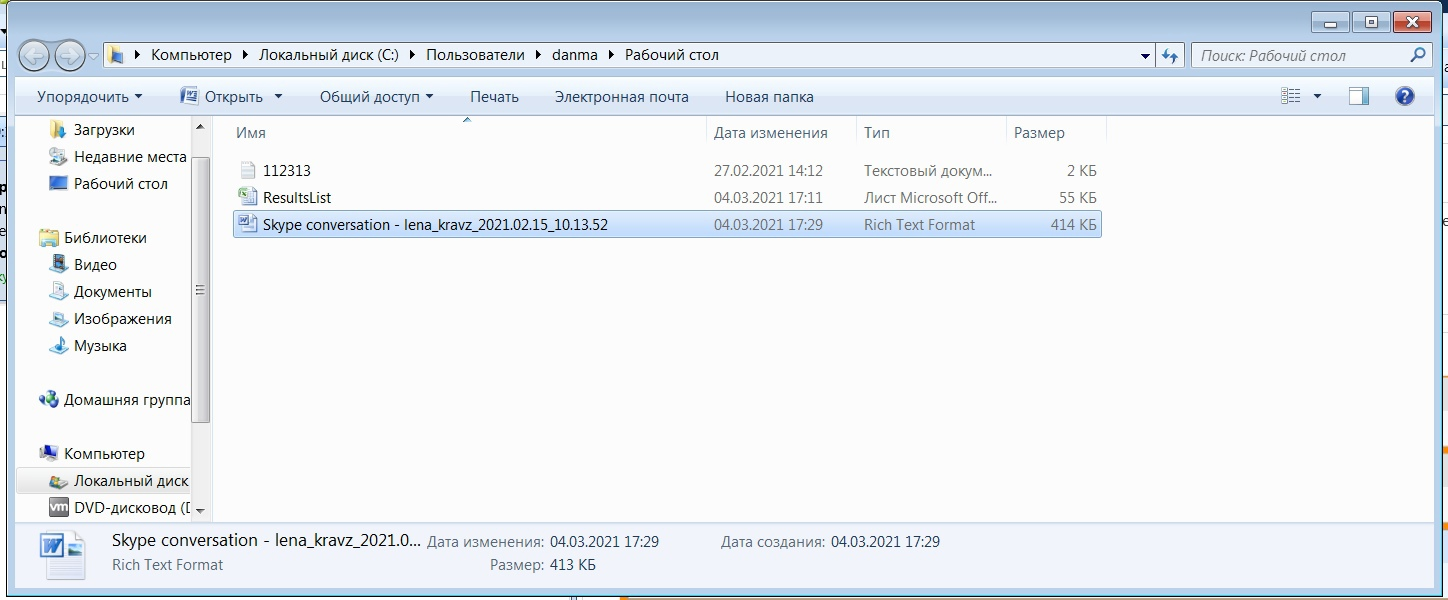
\includegraphics[scale=0.3]{pics/4.7.jpg}

        Файл Skype conversation - lena\_kravz\_2017.09.11\_10.13.52.rtf сохранен
    \end{center}

    \newpage
    \textbf{Пункт 4.11 - Изучите файлы, отправленные в почтовых программах за указанную дату.}
    \begin{center}
        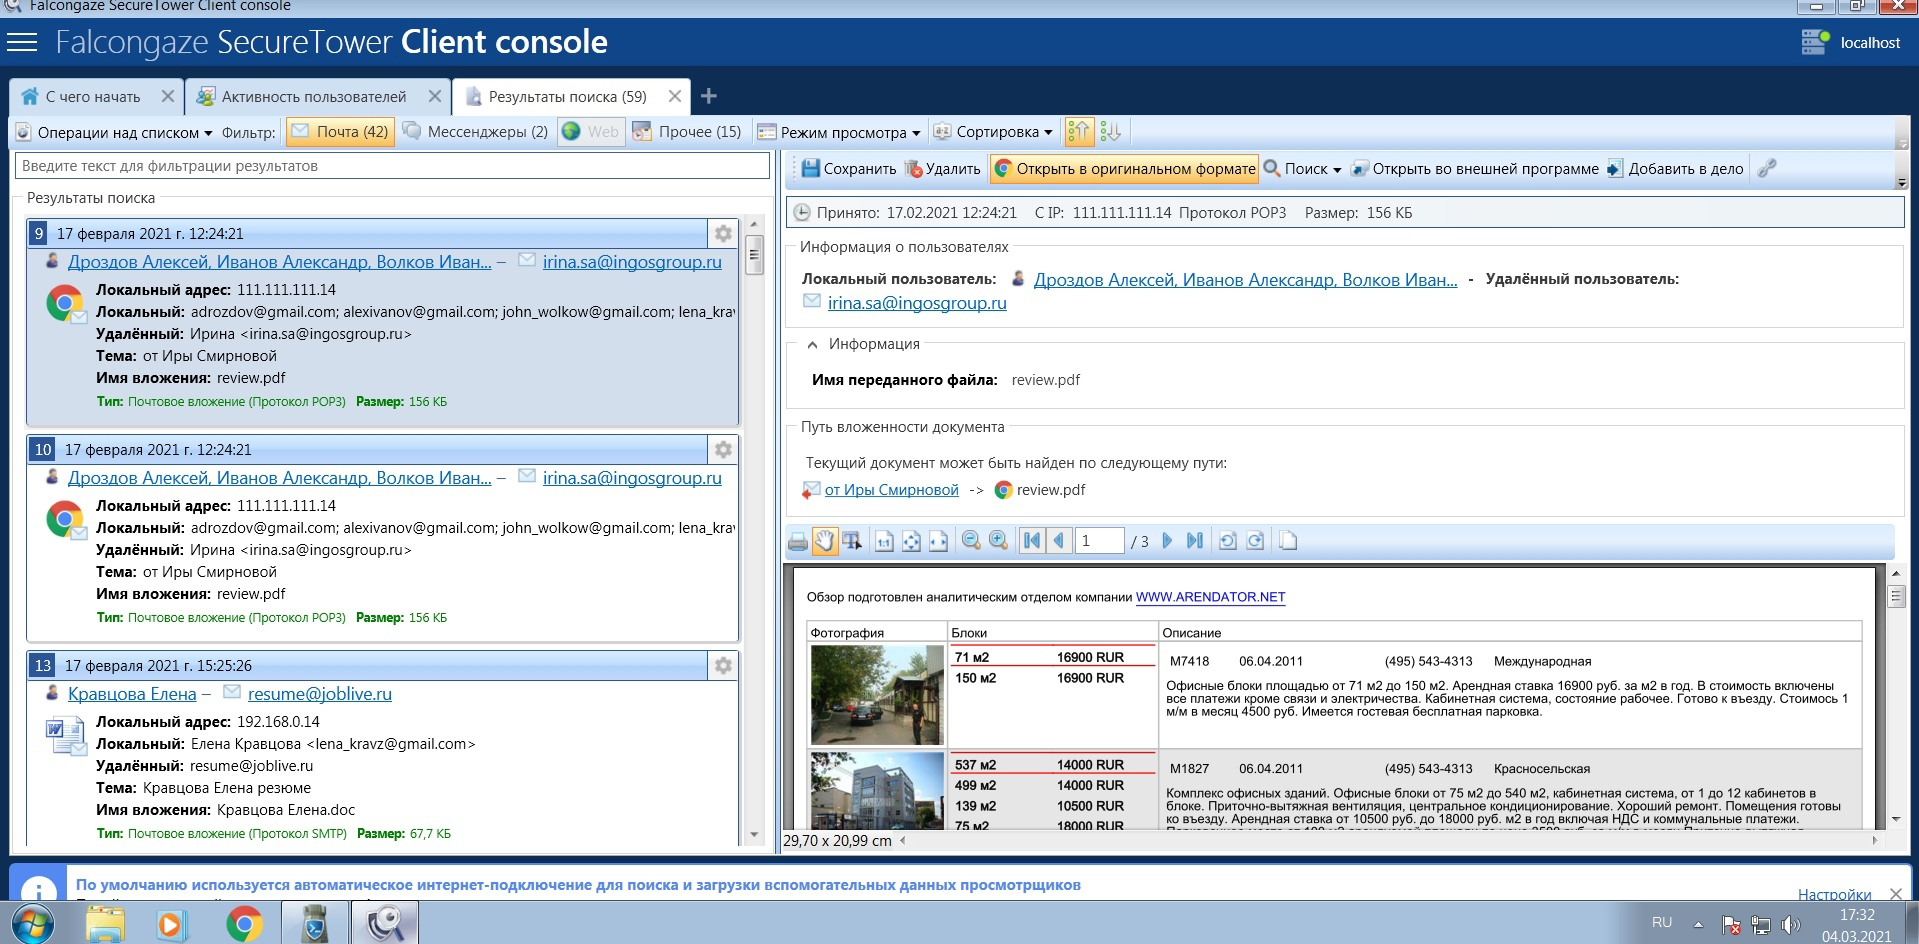
\includegraphics[scale=0.25]{pics/4.11.jpg}

        Результаты поиска.
    \end{center}

    \textbf{Пункт 4.16 - Изучите коммуникации пользователей, контролируемых системой, с
    пользователем Конкурент.}
    \begin{center}
        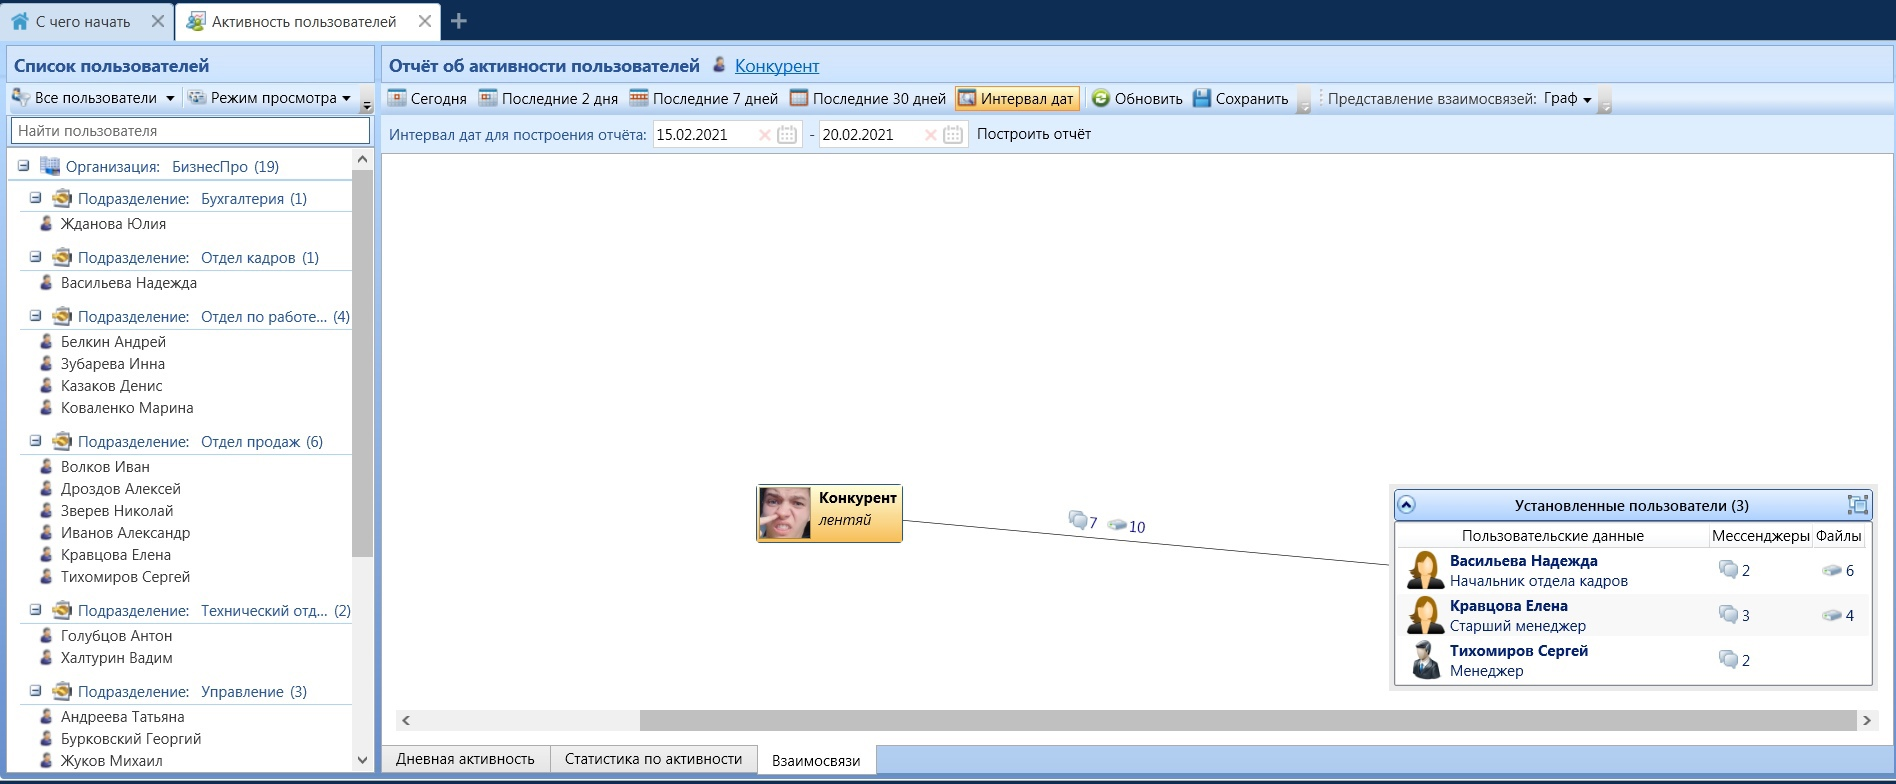
\includegraphics[scale=0.25]{pics/4.16.jpg}

        Коммуникации с конкурентом.
    \end{center}

    \newpage
    \textbf{Выводы:}

    
    \textbf{Ответы на контрольные вопросы.}
    \begin{enumerate}
        \item \textbf{ Чем вызваны различия результатов поиска по ключевой фразе «высылаю
        резюме» при выполнении заданий на шагах 2.2 – 2.5? }

        \qquad Во втором случае включены нечеткий поиск и транслитерация.
        \item \textbf{Какие логические операторы могут применяться для создания поискового
        запроса при комбинированном поиске.}
        
        \qquad И, или, не.
        \item \textbf{ Как отрегулировать интервал. Данные за который должны быть проверены
        на соответствие условиям поискового запроса? }
       
        \qquad  С помощью поля "Интервал дат".
        \item \textbf{Возможно ли создать карточку для нового пользователя через Консоль
        пользователя?}
        
        \qquad  Нет, нельзя.
        \item \textbf{Как быстро проверить все взаимосвязи одного пользователя с другими
        пользователями сети?}
        
        \qquad  "Активность пользователей" -> "Пользователь" -> "Взаимосвязи". 
        \item \textbf{Каковы возможности коммуникаций с внешними контактами и их идентификации?}
        
        \qquad Возможности - отслеживать любой обмен данными (в скайпе, мессенджерах, e-mail и т. д.).
        \item \textbf{ Какие виды активности пользователя отображаются в отчете о дневной
        активности пользователя.}

        \qquad  Переписки, почта, файлы, посещаемые сайты, запускаемые программы и прочее.
   \end{enumerate}
    \end{document}